\documentclass[11pt]{article}

\usepackage[margin=1in]{geometry}
\usepackage{amsmath,amssymb,amsthm}
\usepackage{graphicx}
\usepackage[hidelinks]{hyperref}

\newtheorem{theorem}{Theorem}
\newtheorem{remark}{Remark}

\newcommand{\NA}{\mathrm{NA}}
\newcommand{\Lop}{\mathcal L}
\newcommand{\ext}{\mathrm{ext}}

\begin{document}

\begin{center}
{\Large Literature status: the polyhedral subcase of property \(B\)}

\medskip
{\small Run \texttt{fa\_banach\_001}; source arXiv:1306.1155}
\end{center}

\section*{Source question}

Miguel Martin's paper \emph{Norm-attaining compact operators} asks the
following finite-rank density question.

\begin{figure}[h]
\centering

\includegraphics[width=\textwidth]{figures/open_problem_crop.png}
\caption{Question 9 in arXiv:1306.1155, page 4.}
\end{figure}

\begin{figure}[h]
\centering

\includegraphics[width=\textwidth]{figures/open_problem_continuation_crop.png}
\caption{The following page notes that the problem is open even for the
two-dimensional real Hilbert space.}
\end{figure}

Question 9 asks whether, for every finite-dimensional range space \(Y\) and
every Banach space \(X\), the set \(\NA(X,Y)\) is dense in \(\Lop(X,Y)\).

\section*{Supporting literature status}

The polyhedral finite-dimensional range subcase is already known.  Kadets,
Lopez, Martin, and Werner's 2019 paper \emph{Norm attaining operators of finite
rank} recalls Lindenstrauss's examples of spaces with property \(B\), including
finite-dimensional polyhedral spaces.

\begin{figure}[h]
\centering
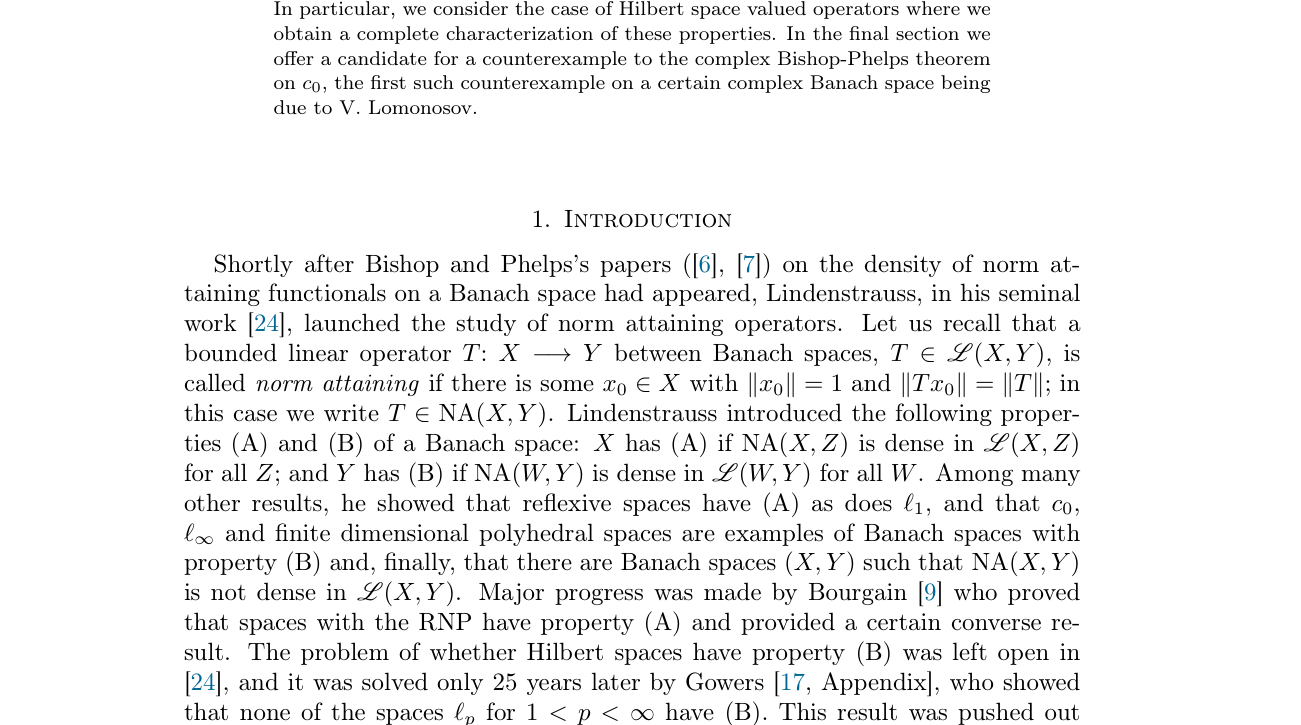
\includegraphics[width=\textwidth]{figures/supporting_polyhedral_known_crop.png}
\caption{arXiv:1905.08272, page 1: finite-dimensional polyhedral spaces are
listed among Lindenstrauss's examples with property \(B\).}
\end{figure}

The same paper also says that the all finite-dimensional version remains a
major open question.

\begin{figure}[h]
\centering
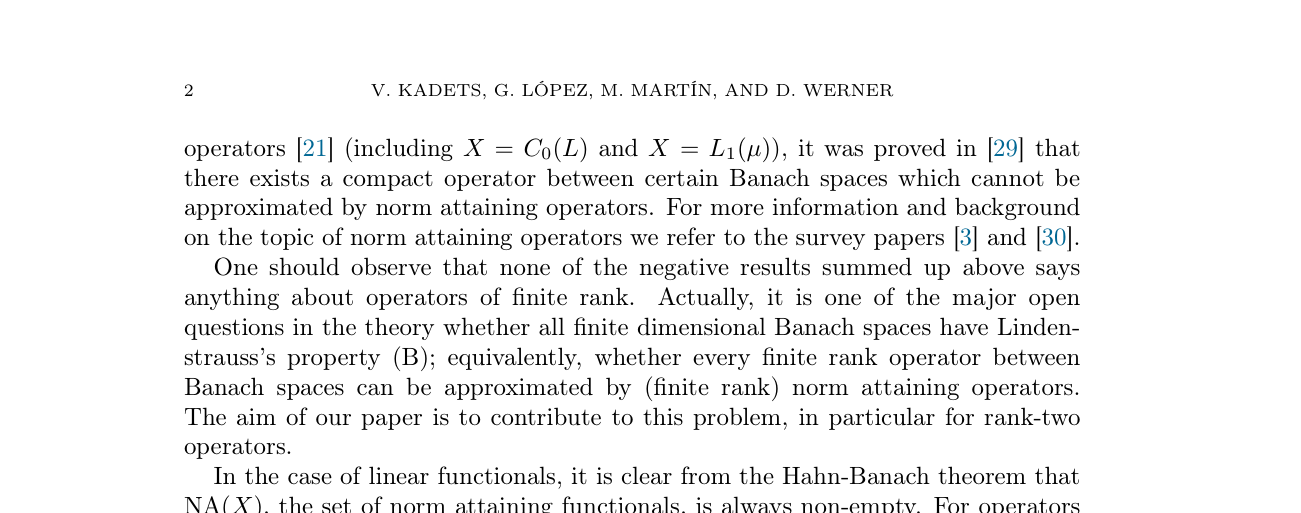
\includegraphics[width=\textwidth]{figures/supporting_full_problem_open_crop.png}
\caption{arXiv:1905.08272, page 2: the full finite-dimensional property \(B\)
problem remains open.}
\end{figure}

Thus the statement below is a literature-known proper subcase of Martin's
Question 9, not a new partial result from this run and not a solution of the
full question.

\section*{Proof intuition for the known subcase}

If \(Y\) is finite-dimensional and polyhedral, then the dual ball
\(B_{Y^*}\) has finitely many extreme points and
\[
  \|y\|=\max_{\phi\in \ext B_{Y^*}} \phi(y).
\]
Hence the norm of an operator \(T:X\to Y\) is the maximum of finitely many
scalar operator norms \(\|\phi T\|\).  Choose an extreme functional
\(\phi_0\) at which this maximum is attained.  Since \(\phi_0\) is a vertex
of a polytope, one can expose it by a vector \(y_0\in S_Y\), so all other
non-opposite extreme functionals have \(|\phi(y_0)|<1\).

The proof then makes the \(\phi_0\)-coordinate slightly dominant and uses the
Bishop--Phelps theorem only in that scalar coordinate.  The exposing gap
prevents all other extreme coordinates from becoming dominant after the small
rank-one correction, so the resulting vector-valued operator attains its full
norm wherever the corrected scalar functional attains its norm.

\begin{theorem}
Let \(Y\) be a real finite-dimensional polyhedral Banach space.  Then for
every real Banach space \(X\), \(\NA(X,Y)\) is dense in \(\Lop(X,Y)\).
\end{theorem}

\begin{proof}
The case \(Y=\{0\}\) is trivial, so assume \(Y\ne \{0\}\).  Let
\[
  F=\ext B_{Y^*}.
\]
Since \(Y\) is finite-dimensional and polyhedral, \(F\) is finite and
symmetric, and \(\|y\|=\max_{\phi\in F}\phi(y)\) for all \(y\in Y\).

Fix \(T\in \Lop(X,Y)\) and \(\varepsilon>0\).  If \(T=0\), then \(T\) itself
attains its norm.  Assume \(T\ne 0\), and put \(M=\|T\|\).  Choose
\(\phi_0\in F\) such that
\[
  \|\phi_0 T\|=M.
\]
Because \(\phi_0\) is a vertex of the polytope \(B_{Y^*}\), there exists
\(y_0\in Y\) exposing \(\phi_0\).  After scaling, we may assume
\[
  \phi_0(y_0)=1
  \quad\hbox{and}\quad
  \phi(y_0)<1 \quad (\phi\in F,\ \phi\ne \phi_0).
\]
Then \(y_0\in S_Y\), and
\[
  c:=\max\{|\phi(y_0)|:\phi\in F,\ \phi\ne \pm\phi_0\}<1.
\]

Choose \(\eta>0\) and \(\delta>0\) so small that
\[
  \eta M+\delta<\varepsilon
  \quad\hbox{and}\quad
  (1-c)\eta M>(1+c)\delta .
\]
By the scalar Bishop--Phelps theorem, there is a norm-attaining functional
\(g\in X^*\) such that
\[
  \|g-(1+\eta)\phi_0T\|<\delta .
\]
Define \(S:X\to Y\) by
\[
  Sx=Tx+\bigl(g(x)-\phi_0T(x)\bigr)y_0.
\]
Then
\[
  \|S-T\|\le \|g-\phi_0T\|
  \le \eta M+\delta<\varepsilon.
\]

Moreover, \(\phi_0S=g\) and \((-\phi_0)S=-g\).  For
\(\phi\in F\setminus\{\pm\phi_0\}\),
\[
  \|\phi S\|
  \le \|\phi T\|+|\phi(y_0)|\,\|g-\phi_0T\|
  \le M+c(\eta M+\delta).
\]
The choice of \(\delta\) gives
\[
  M+c(\eta M+\delta)<(1+\eta)M-\delta\le \|g\|.
\]
Thus
\[
  \|S\|=\max_{\phi\in F}\|\phi S\|=\|g\|.
\]
Since \(g\) attains its norm, choose \(x_0\in S_X\) with
\(|g(x_0)|=\|g\|\).  If \(g(x_0)=\|g\|\), then
\[
  \|Sx_0\|\ge \phi_0(Sx_0)=\|g\|=\|S\|.
\]
If \(g(x_0)=-\|g\|\), replace \(x_0\) by \(-x_0\).  Hence \(S\in\NA(X,Y)\).
Since \(T\) and \(\varepsilon\) were arbitrary, \(\NA(X,Y)\) is dense in
\(\Lop(X,Y)\).
\end{proof}

\section*{Verification notes and limitations}

The proof is purely analytic and uses only the scalar Bishop--Phelps theorem
and the finite exposed-vertex structure of the dual unit ball of a real
polyhedral finite-dimensional space.

This is a literature-known proper subcase of Question 9.  It does not cover real
finite-dimensional spaces with smooth boundary, and in particular does not
cover the two-dimensional real Hilbert space singled out by Martin.  It also
does not treat complex finite-dimensional spaces; the finite-vertex argument is
intrinsically real-polyhedral.

No novelty claim is made.  The supporting literature explicitly records the
polyhedral subcase as known and explicitly says that the full finite-dimensional
problem remains open.

\end{document}
